\section{Pipelined OpenCL BFS overview} \label{sec:overview}
To obtain high-throughput BFS, we pipeline BFS first, which 
enables direct on-chip communication between different 
pipeline stages without going through the shared DRAM.
BFS is a nested loop and each layer of BFS loop is 
converted to a pipeline stage as shown in Figure~\ref{fig:overview}.
The throughput of the pipeline is determined by the 
inner most loop kernel initially. A natural optimization is to duplicate the inner most 
loop kernel spatially. However, memory cannot fulfill the massive 
parallel memory requirements as discussed in Section \ref{sec:motivation}.
Therefore, BFS requires both pipelining optimization and 
memory access optimization. We will focus on BFS pipelining 
optimization in this section and detail memory access optimization 
on top of the pipelining in next section.

Figure \ref{fig:overview} shows the naive mapping strategy 
from original BFS algorithm to hardware pipelines. 
The main processing part is mapped to pipelined OpenCL kernels on FPGAs 
while the control part is done on host CPU due to the lack of 
mechanism to control the pipelined kernels in OpenCL.
Note that $level$ stands for the level of BFS. 
$l$ is the current BFS level and $V$ is the set of graph vertices. 
$v_s$ stands for the source vertex of BFS and is put into the frontier queue initially.
When the level of a vertex is -1, it means the vertex is unvisited yet.
$frontier$ and $next\_frontier$ represent the frontier vertex 
queue of current BFS level and next BFS level respectively.

\begin{figure}
\center{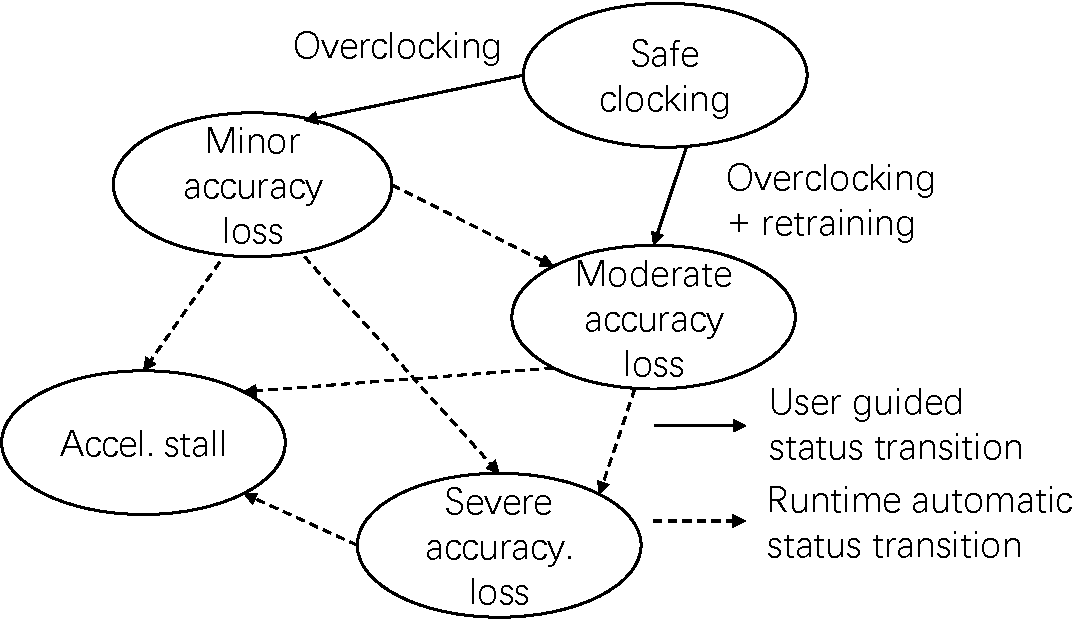
\includegraphics[width=0.65\linewidth]{overview}}
    \caption{Overview of BFS algorithm and hardware pipelining}
\label{fig:overview}
\vspace{-1.2em}
\end{figure}

%The naive mapping is to put each layer of loops to a pipeline stage.
%While more fine-grained pipelining can be beneficial to the processing 
%efficiency and implementation frequency. 
We find that more fine-grained pipelining can be beneficial to the processing 
efficiency and implementation frequency. Thus, we further split the 
inner most loop and divide BFS into five pipeline stages. 
The pseudo code of the BFS with fine-grained pipelining 
is shown in Algorithm \ref{alg:bfs}. Channels are used to connect the different 
pipeline stages. The meaning of each channel can be expected from their names. 
With the fine-grained pipelining, there are no direct dependent memory 
accesses in each pipeline stage. In Stage 1, it reads frontier 
vertices from memory. In Stage 2, 
RPA of the frontier vertices will be read to determine their locations in CIA. 
In Stage 3, it reads CIA array to get the indices of the outgoing 
neighbors. In Stage 4, each neighbor will be inspected and 
unvisited neighbor vertices will be considered as frontier 
in the next BFS iteration. In Stage 5, the new frontier 
vertices will be streamed to memory and the level of 
the frontier vertices will be updated. The five-stage pipeline 
implementation is used as the baseline in this work. 

\vspace{-0.5em}
\begin{algorithm}
	\caption{Pseudo code of pipelined BFS algorithm} \label{alg:bfs}
    \footnotesize
	\begin{algorithmic}[1]
		\Procedure{BFS}{}
		\State $level[v] \gets -1$ where $v \in V$
		\State $level[v_s] \gets 0$
		\State $current\_level \gets 0$
		\State $frontier \gets v_s$
		\State $l \gets 0$

        \While {$!frontier.empty()$} 
		\State $traverseFrontier()$ {//Stage 1}
		\State $inspectFrontierRPA()$ {//Stage 2}
		\State $inspectFrontierCIA()$ {//Stage 3}
		\State $checkNgbVisitStatus()$ {//Stage 4}
		\State $updateFrontier(l)$ {//Stage 5}
		\State exchange $frontier$ and $next\_frontier$
		\State $l \gets l + 1$
		\EndWhile
		\EndProcedure

		\Procedure{$traverseFrontier$}{}
		\For {$v \in frontier$}
		\State $frontier\_channel$.write($v$)
		\EndFor
		\EndProcedure

		\Procedure{$inspectFrontierRPA$}{}
		\State $v \gets frontier\_channel$.read()
		\State {$rpa.start \gets RPA[v]$}
		\State {$rpa.end \gets RPA[v+1]$}
		\State $rpa\_channel$.write($rpa$)
		\EndProcedure

		\Procedure{$inspectFrontierCIA$}{}
		\State $rpa \gets rpa\_channel$.read()
		\For {$idx \gets rpa.start$ to $rpa.end$}
		\State $v\_out \gets CIA[idx]$
		\State $ngb\_channel$.write($v\_out$)
		\EndFor
		\EndProcedure

		\Procedure{$checkNgbVisitStatus$}{}
		\State $v\_out \gets ngb\_channel$.read()
		\If {($level[v\_out] == -1$)}
		\State $next\_frontier\_channel$.write($v\_out$)
		\State $level[v\_out] \gets l + 1$
		\EndIf
		\EndProcedure

		\Procedure{$updateFrontier$}{}
		\State $v\_out \gets next\_frontier\_channel$.read()
		\State $next\_frontier$.write($v\_out$)
		\EndProcedure
	
	\end{algorithmic}
\end{algorithm}
\vspace{-1em}
